
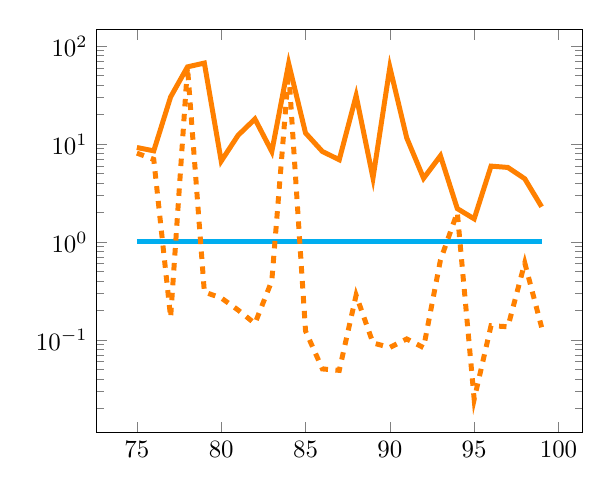
\begin{tikzpicture}[scale=0.9]
\begin{semilogyaxis}
\addplot[color=cyan,line width=2pt] coordinates {(75,1.0)(76,1.0)(77,1.0)(78,1.0)(79,1.0)(80,1.0)(81,1.0)(82,1.0)(83,1.0)(84,1.0)(85,1.0)(86,1.0)(87,1.0)(88,1.0)(89,1.0)(90,1.0)(91,1.0)(92,1.0)(93,1.0)(94,1.0)(95,1.0)(96,1.0)(97,1.0)(98,1.0)(99,1.0)};
\addplot[color=orange,line width=2pt] coordinates {(75,9.21842260217768)(76,8.518374139871337)(77,30.272822753734516)(78,61.38790112141396)(79,67.13758756731826)(80,6.695516853988892)(81,12.279506238234084)(82,18.011628602593053)(83,8.383137070202451)(84,66.41175647549775)(85,12.956334087790534)(86,8.391730265621204)(87,6.912802011120975)(88,31.15096903121106)(89,4.507326282954592)(90,60.71159386109334)(91,11.554421964462923)(92,4.471890566837361)(93,7.5918914094674195)(94,2.190801619524349)(95,1.7224921630136447)(96,5.950743374330171)(97,5.76709428834545)(98,4.418746420771)(99,2.2882968490878937)};
\addplot[dashed,color=orange,line width=2pt] coordinates {(75,8.078058534719021)(76,6.967303633116283)(77,0.16931039226561967)(78,60.92399739469019)(79,0.3077669915726389)(80,0.2683428829493294)(81,0.2016649766255253)(82,0.14692195755641388)(83,0.4007054705663019)(84,55.75434842430663)(85,0.1232959335508722)(86,0.050513749500071196)(87,0.04882301448997559)(88,0.2861979755934838)(89,0.09299299306507139)(90,0.0836608407506848)(91,0.1022671631696554)(92,0.08328271648652821)(93,0.6544187669552102)(94,1.998659777309148)(95,0.024727158057243695)(96,0.13970181933492337)(97,0.1361573781014197)(98,0.6112466149752231)(99,0.1344683724235963)};

\end{semilogyaxis}
\end{tikzpicture}
